\section{Datasets Description}
\label{sec:dataset}
Using \platname, we collected full packet traces from Internet activity generated by
mobile devices. We use this data to study how to map monitored traffic to applications, and to
analyze PII leakage. Below, we describe our data-collection methodology, which consists of
1) controlled experiments in a lab setting and 2) IRB-approved ``in the wild'' measurements 
gathered from real users during seven months.

\subsection{Controlled Experiments}
\label{sec:dataset-contr-exper}
Our goal with controlled experiments is 1) to obtain ground truth information 
about network flows generated by apps and devices, and 2) characterize the 
network activity for a large variety of apps in a lab setting. We use 
this data to understand how to model apps' network behavior, how to map network flows 
to the app that generated them and how to identify PII in those network flows. 

\noindent\textbf{Device setup.} We conducted our controlled experiments using three devices: a Galaxy
Nexus running Android 4.2, a Google Nexus running Android 4.0, and
an iPhone 3GS running iOS 6. We start each set of controlled experiments
 with a factory reset of the device to ensure that software installed by previous 
 experiments cannot impact the network traffic generated by each device. 
 Then we connect the device to the
\platname{} platform, we enable the SSL-Bumping plugin, and begin
the experiment. 

\noindent\textbf{Manual tests.} We manually test the
100 most popular free Android apps in the \emph{Google Play} store and 209
iOS applications from the iOS App store on April 4, 2013. For each
application, we install it, enter user credentials for the account if
it is relevant, interact with it for up to 10 minutes, and uninstall
it. This allows us to characterize real user interactions with popular applications 
in a controlled environment. Note that 
because we enter a unique and distinguishable set of user credentials when 
interacting with apps, we can easily extract the corresponding PII from 
network flows (if they are not obfuscated).

\noindent\textbf{Automated tests.} The second set of controlled experiments consist of fully-automated
experiments on the most popular 732 Android applications from a free,
third-party Android market, \emph{AppsApk.com}~\cite{appsapk}.
We perform this test because Android devices can install
\emph{Third-party applications} that are not available on the
\emph{Google Play} store, without requiring the user to root the device. 

Our goal is to understand how these apps differ from those in the standard \emph{Google Play} 
store, as they are not subject to Google Play restrictions.
%\tbd{Is there different constraints on this free market, AR: They do not have paid application. All apps must be free.}
We automate experiments using \emph{adb} to
install each app, connect the device to the \platname{} platform, and
start the app. Then we use \emph{Monkey}~\cite{adbmonkey}, an app-scripting 
tool, to perform a series of 10,000 actions \drc{Is it still the case that we have 10k actions?} that include
random swipes, touches, and text entries.  Finally, we use adb to
uninstall the application and reboot the device to forcibly end any
lingering connections. This set of experiments is limited to
Android devices because iOS does not provide equivalent 
scripting functionality. 

% The results of our controlled experiments can be found in
% \fref{sec:manual-testing}.

\subsection{In The Wild Measurements}
\label{sec:dataset-wild-measurements}

The controlled experiments in the previous section provide us with 
ground-truth information for a large number of apps running in a controlled 
setting for a short period of time. To understand the network behavior of 
devices with real users "in the wild" over longer time periods, we conducted 
an IRB-approved measurement study with a small set of subjects, from 
Oct. 15, 2012 to Sep. 01, 2013.\footnote{The measurement study is ongoing, we report the most recent subset of results.}

We deployed two \platname servers, one in the USA and one in France
that were used by 26 devices: 10 iPhones, 4 iPads, 1 iPodTouch, and 11
Android phones.  The Android devices in this dataset include the
Nexus, Sony, Samsung, and Gsmart brands while the iPhone devices
include one iPhone~3GS, four iPhone~5, and five iPhone~4S.  These
devices belongs to 21 different users, volunteers for our IRB approved
study.  This dataset, called \mobWild, consists of 318 days with data; the number of 
days for each user varies from 5 to 315 with a median of 35 days.  For privacy reasons, the
SSL-Bumping plugin is \emph{disabled} for all measurements involving
real users.

Capturing all of a subject's Internet traffic raises significant
privacy concerns.  Our IRB-approved study entails informed consent
from subjects who are interviewed in our lab, where the risks and
benefits of our study are clearly explained.  The incentive to use
VPNs is Amazon.com gift certificates awarded by lottery. To protect the
identity of information leaked in the data, we use public key
cryptography to encrypt all data before storing them 
on disk; the private key is
maintained on separate secure severs and with access limited to
approved researchers.  Further, subjects are free to delete their
data and disable monitoring at any time.  Per the terms of our IRB, we cannot 
make this data publicly available due to privacy concerns. We are investigating 
alternative data-collection techniques that provide user anonymity sufficient 
for sharing with other researchers.

\section{Analysis of Mobile Network Flows}
In this section, we analyze the network traces gathered by \meddle to 
1) provide summary statistics of data gathered from our 
users ``in the wild'' and
2) develop and evaluate several techniques for mapping network flows to 
applications, which we will use in subsequent sections to identify privacy 
leaks and malware.


\subsection{Descriptive Statistics from User Study}

This section highlights key features of the dataset gathered from 
users participating in our study (\mobWild). 
Due to the relatively small number of users in our study, we cannot 
draw strong, generalizable conclusions; rather, we use data gathered 
from them to demonstrate that there is a need for \platname{} to 
obtain a comprehensive view of Internet traffic from mobile devices. 

\noindent\textbf{Observation 1: \emph{Devices use a variety of networks and use each differently.}} First, we describe the diversity 
of networks that our users connected to. 
We infer the access technology (WiFi or cellular) using the AS description from \emph{WHOIS} data for each IP address used by a mobile device.
Based on this classification, the \mobWild dataset consists of traffic from 65 distinct ASes\drc{How many are academic?}, of which 8 are cellular ASes.
\tbd{AR: 7 of these ASes belong to Universities -- however if the university is being served by an ISP then I cannot identify it}
During the measurement study, each device connected to our \platname server from at most two distinct cellular ASes. 
In contrast, a median of 4 \wifi ASes were observed per device and for one device we observed traffic from 36 different \wifi ASes spread across 5 countries.
In terms of traffic volumes, collectively our users' \tbd{AR: who used a cellular data plan for their} devices transferred 24-56\% of their traffic over cellular \tbd{AR: (iOS and Android, respectively) -- remove iOS and Android}, and the 
remainder over WiFi. 
The key take-away is that, \emph{for our users}, instrumenting a single cellular carrier or WiFi access point misses a 
large fraction of traffic generated by mobile devices. \platname{} avoids this limitation.

\noindent\textbf{Observation 2: \emph{Most traffic is HTTP(S), and the dominance of SSL can hinder traffic visibility}.} We begin our identification process using the classification provided Bro~\cite{bro}.
Bro uses the protocol field in the IP header to broadly classify the flows, and we use this classification to label flows as either TCP, UDP, or \emph{other}.
Bro further classifies TCP flows using well defined port numbers, and we use this classification to label flows as either HTTP, SSL (which includes HTTPS, IMAP, etc.) or \emph{other} flows.
Similarly, we use Bro to label UDP flows as either DNS or \emph{other}. 
Table~\ref{tab:summaryIOSAndroidTraffic} presents a 
summary of traffic generated by user devices in our study. 

There are two key  
take-aways from this table. First, Web and SSL traffic dominate traffic for users in \mobWild, 
and there is significant diversity in the usage patterns for 
users with Android and iOS devices. For example, more than 92\% of the traffic\drc{volume?} in our \mobWild dataset is either HTTP or SSL, 
the fraction of total flows over cellular or \wifi differ significantly for each OS. This motivates the need for a platform that covers 
multiple OSes and multiple access technologies. Second, a significant portion of flows occur over secure (SSL) connections 
that generally prevent classification using deep packet inspection. This calls into question 
the overall effectiveness of traffic optimization approaches that rely 
on middlebox technologies that interpose of plaintext traffic (\eg page rewriting or downsampling media).

\begin{table}
\begin{small}
\begin{center}
\begin{tabular}{|p{0.11\columnwidth}|p{0.14\columnwidth}|r|r|r|r|}
\hline
{\bf IP} & \multirow{2}{*}{\bf Service} & \multicolumn{2}{|c|}{\bf Android} & \multicolumn{2}{|c|}{\bf iOS} \tabularnewline
\cline{3-6}
{\bf Protocol} &           &  \textbf{Cell.}  &  \textbf{\wifi}  &  \textbf{Cell.}  &  \textbf{\wifi}  \tabularnewline
\hline
\multirow{3}{*}{TCP}
       &  HTTP (\%)  & 35.39 & 68.67 & 52.11 & 75.51 \tabularnewline
\cline{2-6}
       &  SSL (\%)   & 61.14 & 27.37 & 46.76 & 18.76 \tabularnewline
\cline{2-6}
       &  other (\%) & 2.34  & 3.29  & 0.26  & 1.81 \tabularnewline
\hline
\multirow{2}{*}{UDP}
       &  DNS (\%)   & 0.67  & 0.49  & 0.56  & 0.34  \tabularnewline
\cline{2-6}
       &  other (\%) & 0.32  & 0.11  & 0.27  & 3.57  \tabularnewline
\hline
 Other &  other (\%) & 0.14  & 0.07 & 0.04  & 0.01  \tabularnewline
\hline
\multicolumn{2}{|c|}{\emph{total (\%)}} & 100.00 & 100.00 & 100.00 & 100.00 \tabularnewline
\hline
\multicolumn{2}{|c|}{\emph{Traffic Volume (GB)}}& 9.467 & 18.79 & 14.89  & 89.54 \tabularnewline
\hline
\multicolumn{2}{|c|}{\emph{\# Flows}}   & 851074 & 658331 & 661736 & 2167448 \tabularnewline
\hline
%\multicolumn{2}{|c|}{\emph{\# Devices}} & 10 & 11 & 10 & 15 \tabularnewline
%\hline
\end{tabular}
\end{center}
\end{small}
\caption{\tbd{AR: Update Table}Traffic volume (in percentage) of popular protocols and services on Android and iOS devices over cellular and \wifi.
\emph{TCP flows are responsible for more than 90\% of traffic volume. Traffic share of SSL over cellular networks is more than twice the traffic share of SSL over \wifi.}} 
\label{tab:summaryIOSAndroidTraffic}
\end{table}

An important question for network characterization is which app is responsible for which 
network flows. As we demonstrate in the following section, previous approaches are insufficient 
for mapping the majority of apps to their corresponding network flows. We describe 
several techniques to improve this mapping, and present results for controlled experiments 
and the \mobWild dataset.


\subsection{Mapping Network Flows to Apps}
%\section{Traffic Classification}
\label{sec:classification-methodology}

In this section, we revisit mobile traffic characterization and classification, using a comprehensive 
view of Internet traffic from mobile devices. The following sections show that  \emph{previous approaches to classifying passively gathered traffic fail to identify
apps responsible for that traffic most of the time} and that \platname{} facilitates a first look at 
determining which apps generate traffic over SSL connections.

%Previous work uses passively gathered data 
%to characterize such traffic, which can be useful for a variety of important topics that include 
%traffic engineering, optimization of network-enabled apps and understanding threats to user privacy. 


% 1) for the users in our study, traffic over WiFi and cellular networks 
%are qualitatively different, and studies that focus on only one technology will miss approximately 
%half of the traffic generated by devices; 

%\subsubsection{Classification of Mobile Apps and Services}

Our \mobWild dataset suggests that apps, OS services and libraries often rely on HTTP and SSL to exchange data~\cite{maier:mobtraffic,falaki:mobileusage,xu:appusage}.
%To analyze the behavior of mobile services we need to first associate the observed flows with the applications and the OS services responsible for the flows.
In the following analysis, we focus on identifying the apps, OS services, and other services responsible for these HTTP and SSL flows. 
We use ground-truth data from controlled experiments to show that the previous approach for classification fails 
for most popular apps; we then develop techniques to improve this mapping and apply it to our \mobWild dataset. 

\subsubsection{Improving HTTP Traffic Classification}

\drc{Update with Ashwin's thesis?}
Mapping network flows to apps is an important step for determining the origins of potentially costly 
network traffic, and for identifying which apps are responsible for privacy leaks. One approach for this is to use the \useragent field on app-generated traffic.
Previous work uses this to classify traffic, but only at the granularity of the app category~\cite{erman2011http,xu:appusage,maier:mobtraffic}. 
Below we describe the limitations of this approach for a large fraction of apps, and how we improve classification using only header information (\ie HTTP and lower layers). 
%use the results from our controlled experiments and the \mobWild dataset to argue that the \useragent can be used to identify flow from popular iOS and Android applications, for flows that do not contain a useful \useragent we fall back to classifying identifying the web-service using the \httphost field.

To motivate why this is a difficult problem, consider the following scenario. When using the \httphost field in the HTTP header, a flow with \emph{static.ak.fbcdn.net} in the \httphost field implies that it contacted one of the Facebook servers; however, the \httphost field does not tell us whether Facebook is accessed via a Web browser or through the native Facebook app. Similarly, the \useragent field can specify an app name, but it is not required to do so. Below, we show the effectiveness of combining these approaches. 


%\begin{table} 
%    \begin{small}
%    \begin{tabular}{|p{0.1\columnwidth}|p{0.18\columnwidth}|p{0.1\columnwidth}|p{0.13\columnwidth}|p{0.17\columnwidth}|}
%       \hline
%       {\bf OS}& {\bf Store} &{\bf \# Apps}&{\bf Generated HTTP}& {\bf Correct User-Agent} \tabularnewline
%       \hline    
%       iOS     & App Store   & 209 & 176 & 149 (84.6\%) \tabularnewline
%       Android & Google Play & 100 & 92  & 21 (22.8\%)  \tabularnewline
%       Android & Third party & 908 & 494 & 32 (6.4\%)   \tabularnewline
%       \hline
%    \end{tabular}
%    \end{small}
%    \caption{Classification of applications based on \useragent. \emph{We observe that we were table to classify \tbd{} of iOS and \tbd{} of Android applications that generated traffic during our experiments.}}
%    \label{tab:classification-success}
%\end{table}


\begin{table} 
     \centering
     \begin{small}
     \begin{tabular}{|p{0.05\columnwidth}|p{0.08\columnwidth}|p{0.07\columnwidth}|p{0.08\columnwidth}|p{0.09\columnwidth}|p{0.09\columnwidth}|p{0.09\columnwidth}|p{0.09\columnwidth}|}
        \hline
        {\bf OS}&{\bf Store}&{\bf Apps}&{\bf Gen.}&\multicolumn{2}{|c|}{\bf Host} & {\bf User-}&{\bf Combi-} \tabularnewline
        \cline{5-6}    
             &        &     & {\bf HTTP} & {\bf App. } & {\bf Org.}& \bf{Agent}   & \bf{nation}  \tabularnewline                
        \hline    
        iOS  & Apple  & 209 & 176 & 83 (47.1\%)  &  119 (67.6\%)   &  149 (84.6\%)& 157 (89.2\%) \tabularnewline
        \hline
        And. & Google & 100 & 92  & 41 (44.5\%)  &  54 (58.6\%)    &  21 (22.8\%) &  59 (64.1\%)  \tabularnewline
        \hline    
        And. & Other  & \tbd{} & 491 &  (...\%) &  (....\%)     &  (....\%)  &  163 (....\%)  \tabularnewline
        \hline
     \end{tabular}
     \end{small}
     \caption{Classification of apps based on \httphost and \useragent. \emph{A large majority of iOS apps use dedicated \useragent strings to fetch data over HTTP. A combination of \useragent and \httphost can be used to identify the majority of Android and iOS apps.} }
     \label{tab:classification-success}
\end{table}

%%
%% No HTTP Traffic from 209 - 38 = 171; 171 + 5 (OS possibly - confirm) = 176  ,
%% 181 unique signature, 7*2 = 14 duplicate (fooducate, fdct). 
%% 174 unique application signatures found
%% 5 UA belonged to OS services, geoservices, applecoremedia, gamekit, securityd, mmsdk 
%% Ads from 98 - 4 -> 94 labels
%% Rough estimate of HTTP for apps because mapping  -- 414 files without HTTP
%%%
%% 217 of the 419 apps that generated traffic generated some ad traffic. 


\noindent\textbf{Controlled experiments.}
In Table~\ref{tab:classification-success} we present results from our classification study using controlled experiments. To 
the best of our knowledge, we are the first to attempt to use ground-truth information to evaluate the 
effectiveness of app classification using only header data.
 

\emph{iOS:}
First, we note that 176 of the 209 iOS apps we manually tested generated HTTP traffic.
We observe that the \httphost field uniquely identified the corresponding app for 47\% of the iOS apps we tested (column 5).
%; the flows containing the application signature was responsible from 15\% to 98\% of the traffic volume from the application. 
%\tbd{TODO: This was done only for a sample of applications -- I shall perform this test in detail after deadline}
The \httphost field also can identify the provider that released an app.
For example Zynga offers multiple games with dedicated apps that contact Zynga properties.
When classifying apps according to their provider, we observe in Table~\ref{tab:classification-success} (column 6) that our classification success increases to 67\% of iOS apps. 


\emph{Android:} We observe similar results for flows from apps released through Google Play.
However, for the apps from the Third-party store we observe that the \httphost field is less effective. 
Primarily this is due to the fact that a majority of the apps we tested (about 77\%) were stand-alone services such as games where the provider did not use its own Web service. Instead, these apps either contacted some advertisement sites or sites hosted by CDNs. 
While we can use the \httphost field to identify these 3rd-party sites contacted by an app, we cannot determine which app generated the traffic. 

\begin{table}
\begin{small}
\begin{tabular}{|l|p{0.85\columnwidth}|}
\hline
{\bf No. } & {\bf User-Agent}\tabularnewline
\hline
1 & YahooMobileMail/1.0 (Android Mail; 1.4.6) (crespo;samsung;Nexus S;4.1.2/JZO54K)\tabularnewline
\hline
2 & AppleCoreMedia/1.0.0.10A523 (iPad; U; CPU OS 6\_0\_1 like Mac OS X; en\_us) \tabularnewline
\hline
3 & Dalvik/1.6.0 (Linux; U; Android 4.2.2; Nexus 4 Build/JDQ39) \tabularnewline
\hline
\end{tabular}
\end{small}
\caption{Sample \useragent strings. \emph{The first string contains the app identifier, the second hides the app and describes the OS service/library used, while the third does not contain any useful signature.}}
\label{tab:user-agent}
\end{table}

\emph{Augmenting with \useragent: } We now show that by augmenting the information in the \useragent to the information gained by the \httphost field, we can classify a majority of iOS and Android apps. 
In our controlled experiments we observed a non-empty \useragent string in more than 99.7\% of the HTTP flows from iOS and 90.9\%flows from Android. 

A \useragent string may contain an app identifier and other auxiliary information such as details of the OS, manufacturer, and compatibility with Web browsers~\cite{mozilla:useragentdetection}. 
For example, the first \useragent in Table~\ref{tab:user-agent} contains the information of the app, YahooMobileMail, while the second \useragent hides the app and specifies the \emph{AppleCoreMedia} service of iOS, and the third does not provide any useful information. 
To extract the app information, we use a set of regular expressions to filter out the auxiliary information in the \useragent and further cluster these extracted tokens using the edit distance between the tokens.\footnote{We plan to release this code along with \platname package.}

In Table~\ref{tab:classification-success} we observe that 176 of the 209 iOS apps generated HTTP traffic, 149 of these were correctly identified based on the signatures in their \useragent, which we verified by manual inspection.
In contrast, our \useragent based identification was able to correctly identify less than 23\% of the Android apps that generated HTTP traffic. 
For the 27 iOS apps which we failed to identify, we observed signatures for OS services and libraries, such as \emph{Apple Core Media}, \emph{Game Kit}, \emph{Geo Services}, etc. and signatures of third-party libraries and services such as \emph{Google Analytics} and \emph{Adobe Air}.
Similarly, the majority of Android HTTP traffic contained flows with the default \useragent (similar to the third \useragent in Table~\ref{tab:user-agent}).
Further, for the apps from the third-party store, we observe that the \useragent for ads and analytics libraries such as \emph{Google Analytics} and \emph{Adsense for Mobile} were the most common \useragent after the default \useragent.

To wrap up, \useragent is more effective for classifying iOS apps and \httphost is more effective for Android apps; however, neither alone is a complete 
solution. A topic of future work is to explore packet contents using deep packet inspection -- it is likely that apps are identifying themselves to CDNs and 
ad/analytics servers in the payload. 

\begin{figure}
\subfloat[iOS]{\label{fig:http-wordcloud-ios}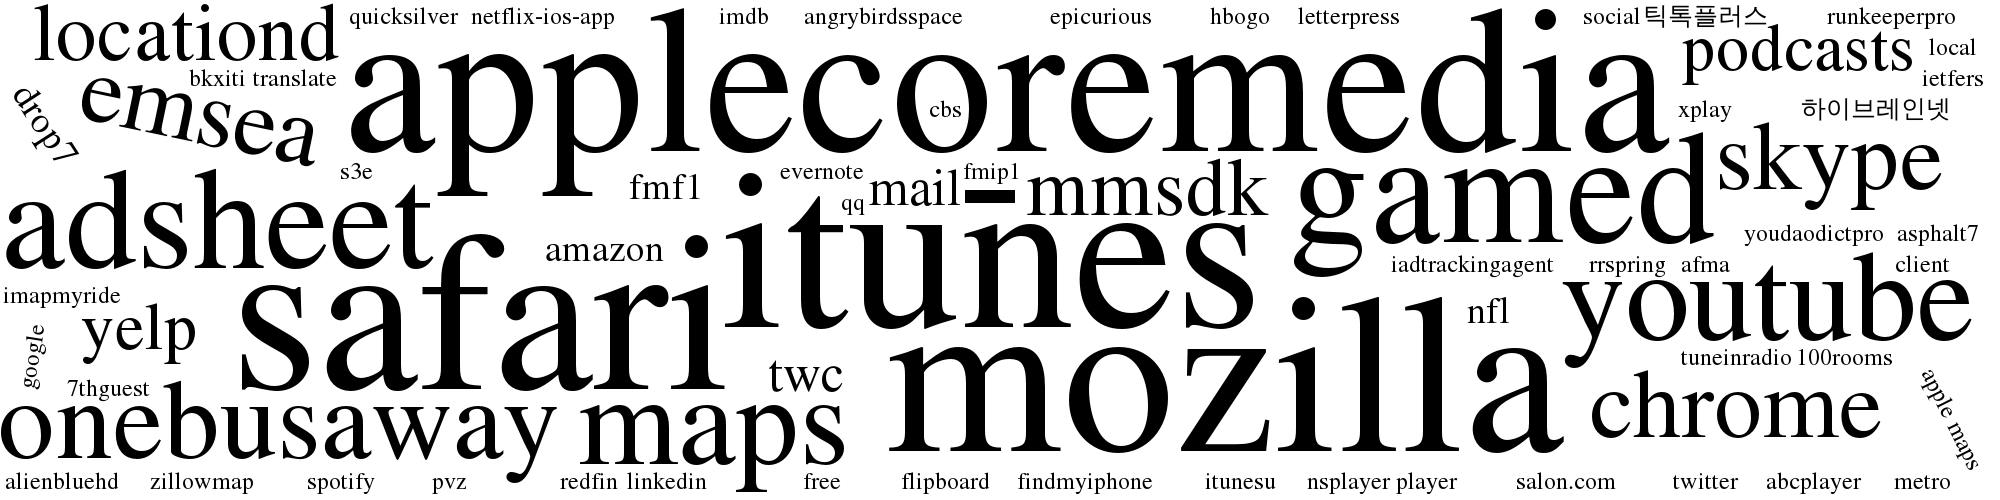
\includegraphics[width=\columnwidth]{figures/wordcloud_useragentsignature_ios_image.png}}\newline
\subfloat[Android]{\label{fig:http-wordcloud-android}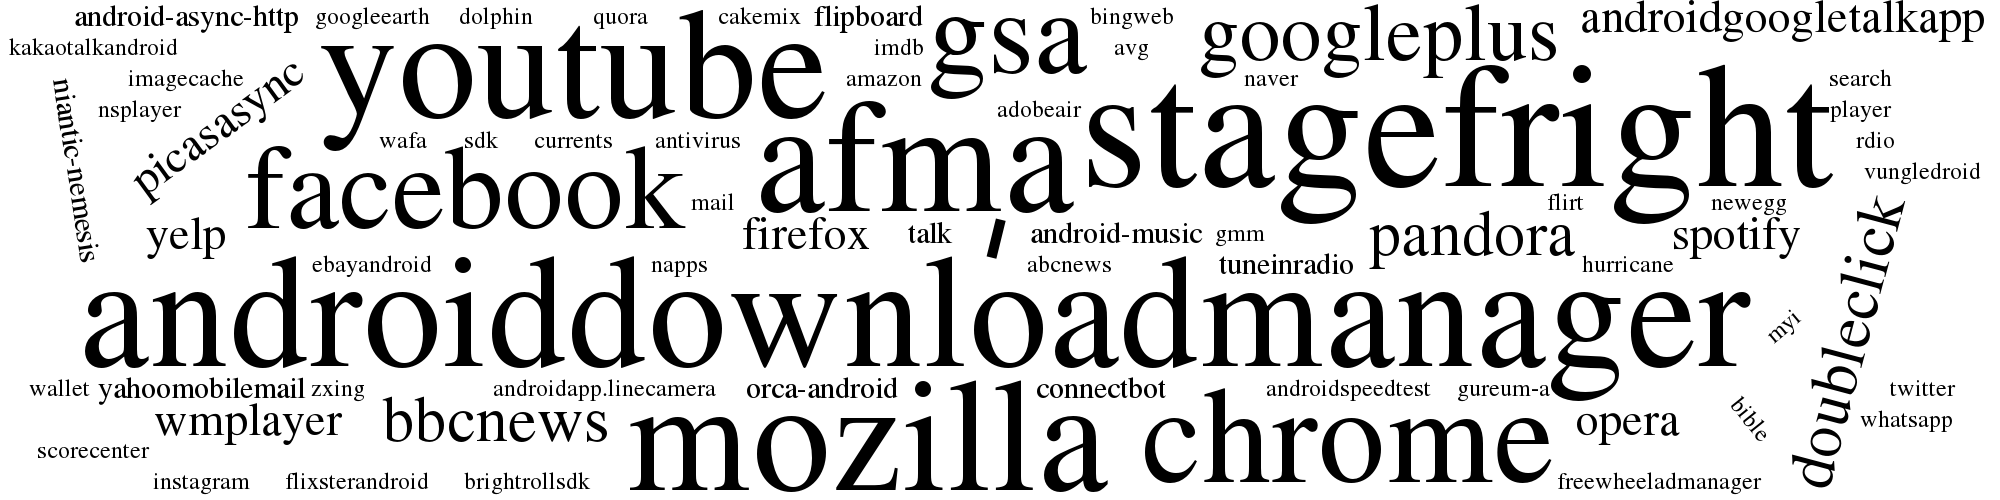
\includegraphics[width=\columnwidth]{figures/wordcloud_useragentsignature_android_image.png}}
\caption{\useragent signatures in  iOS and Android HTTP flows. \emph{The font weight represents the number of users for which a particular signature was observed.}}
\vspace{\postfigspace}
\label{fig:http-wordcloud}
\end{figure}

\textbf{In the wild data.}
We now describe the results of our classification on data gathered from our user study.
Using only the \useragent on the \mobWild dataset we were able to map flows to 243 iOS and 84 Android apps, OS libraries, and services. 
The \emph{word cloud} in Figure \ref{fig:http-wordcloud} contains the summary of our results; the font size of a signature is proportional to the number of users for which the signature was observed.
Along with signatures of apps such as iTunes and YouTube, we also observe signatures of the \emph{Apple Core Media} and \emph{Stagefright} services that are responsible for downloading media content on iOS and Android devices respectively.
%Across the iOS and Android devices, we observe a total of \tbd{1435} unique \useragent strings that produce \tbd{361} unique signatures which we cluster to \tbd{} different apps and services. 
For the iOS devices in the \mobWild dataset, we observe a signature of \emph{Apple Core Media} in more than 98.45\% of the content downloaded from the YouTube servers.
Similarly, depending the Android version we observe either the signature for Stagefright or no app or OS service signature for YouTube traffic to Android devices depending on the OS version. 
We observe a similar signatures for other popular media services such as Netflix, YouTube, Vimeo, Pandora, etc.
Because we cannot identify the app used to access these services, we fall back to the \httphost field to identify these Web services.

\begin{table}
\centering
\begin{small}
\begin{tabular}{|p{0.25\columnwidth}|c|c|c|c|}
\hline
\multirow{2}{*}{\bf Category} & \multicolumn{2}{c|}{\bf \% of iOS Traffic } &  \multicolumn{2}{c|}{\bf \% of Android Traffic } \tabularnewline
\cline{2-5}
  & {\bf Bytes}  & {\bf Flows} & {\bf Bytes} & {\bf Flows}   \tabularnewline
\hline
Media (Popular)         & 51.405  & 12.131 & 65.922 & 22.377 \tabularnewline
\hline
Application             & 33.987  & 80.758 & 31.353 & 77.498 \tabularnewline
\hline
Media (Other)           & 14.572  &  5.914 &  2.712 &  0.044 \tabularnewline
\hline
Other                   &  0.036  & 1.1963 &  0.013 &  0.081 \tabularnewline
\hline
{\em total}             & 100 (\%)& 100 (\%)& 100 (\%) & 100 (\%) \tabularnewline
\hline
\end{tabular}
\end{small}
\caption{Classification of HTTP Traffic. \emph{Popular media services such as Netflix and YouTube dominated the traffic volume, responsible for more than 80\% of iOS and 77\% of Android HTTP flows.}}
\label{tab:classify-http}
\vspace{\postfigspace}
\end{table}

In Table~\ref{tab:classify-http}, we observe that with a combination of \useragent and \httphost field in HTTP headers, we were able to classify more than 98\% of the traffic in terms of flows and bytes from iOS and Android devices.
We observe that media from popular hosts in our \mobWild dataset, including Netflix, YouTube, Pandora, Spotify, and Vimeo, contribute to more than 50\% of the traffic volume from iOS and Android devices.
Similarly, we observe that apps identified based on the \useragent  were responsible for more than 77\% of flows from Android and iOS devices. 
We also observe that media (identified based on the signatures such as \emph{Apple Core Media} and \emph{Stagefright}) served from CDNs and others hosts from which we could not identify the Web service from other fields in the HTTP header, and also the DNS responses before the HTTP flows, comprises 14.5\% of the traffic volume for the iOS devices in our dataset.

\subsubsection{SSL Traffic Classification without Decryption}

Unlike HTTP flows, SSL flows provide limited information in plaintext that can be used to identify the apps. 
For the traces captured during our controlled experiments, we use SSL bumping to classify HTTP flows using 
the techniques described in the previous section. 
However, we did not perform SSL bumping for the devices in the \mobWild dataset, so we now describe how to 
classify SSL flows \emph{without decryption}. 
%As we show below, we used the port number, the SSL certificate with server 
%name identification, and DNS queries to identify the source of SSL traffic. 

% \begin{table}
% \centering
% \begin{small}
% \begin{tabular}{|p{0.25\columnwidth}|c|c|c|c|}
% \hline
% \multirow{2}{*}{\bf Service} & \multicolumn{2}{c|}{\bf iOS} &  \multicolumn{2}{c|}{\bf Android} \tabularnewline
% \cline{2-5}
%   & {\bf Bytes}  & {\bf Flows} & {\bf Bytes} & {\bf Flows} \tabularnewline
% \hline
% HTTPS                   & 91.287 & 81.960 & 97.852 & 97.168    \tabularnewline
% \hline
% Mail                    &  6.700 & 15.872 & 0.689  & 0.320  \tabularnewline
% \hline
% Notification            &  1.412 & 1.553  & 1.321  & 2.100  \tabularnewline
% \hline
% Other                   &  0.601 & 0.615  & 0.138  & 0.412 \tabularnewline
% \hline
% {\em total}             & 100 & 100 & 100 & 100 \tabularnewline
% \hline
% \end{tabular}
% \end{small}
% \caption{Classification of SSL Traffic based on port number. \emph{HTTPS is the most popular service that uses SSL in the \mobWild dataset.}}
% \label{tab:classify-ssl-port}
% \end{table}

Mobile devices use SSL for various services including mail, notifications, instant messaging, and Web browsing.
Services such as mail, instant messaging, and notifications are documented to use dedicated port numbers of their traffic.
%\footnote{We also use the AS for identifying push notification messages as detailed in \fref{sec:characterize-os}.}
Using port numbers, we observe in that more than 99\% of the SSL flows observed in our controlled experiments were due to HTTPS, the rest of the flows were due to email, instant messaging, and OS notification services. 
We therefore focus our attention on identifying the Web services responsible for the HTTPS flows. 

%\tbd{THE NUMBERS FOR THIS ARE FROM THE WILD MEASUREMENTS. ON SIMPLE GLANCING I WAS ABLE TO OBSERVE SIMILAR NUMBERS. I SHALL ADD THEM BY THE TIME OF THE CAMERA READY}

\noindent\textbf{Classification techniques.} We first use the common name (CN) field of certificates to identify the servers that exchanged data using HTTPS.
We observe that less than 25\% of the HTTPS traffic from iOS and Android contains the fully qualified domain name (FQDN) in the subject of the certificate; the rest of the traffic either contains regular expressions such as *.google.com in the certificate.
% or is a continuation of a previous SSL session. 
To further resolve the hostnames, we rely on \emph{server name indication} used by SSL flows~\cite{rfc:servernametls}.
Servers that host multiple services use the \emph{server name indication} to distinguish these services.   
For example, we observe a \emph{server name indication} of \emph{plus.google.com} and \emph{s.youtube.com} in two flows that used a certificate with a CN \emph{*.google.com}.
However, we observe that by using either the certificate or the \emph{server name} we were able to identify the name of the Web service in less than 40\% of iOS and Android HTTPS traffic.

\noindent\textbf{DNS mapping.} For the remaining flows we use DNS requests made by the mobile devices before starting the HTTPS flows, a technique similar to DN-Hunter~\cite{bermudez:dnhunter}.
DN-Hunter relies on the most recent FQDN that corresponds to the IP address, however in our controlled experiments we observe Android and iOS devices use the first entry in DNS response while resolving \emph{hostnames}.
We therefore use the latest DNS response that contains the IP address of the Web service in the first position of the DNS response. 
%FOR THE WILD: Indeed, for 97.8\% of the Android and 83.4\% of the iOS HTTPS traffic that we could not classify using other fields, we observe that the latest DNS response before the flow started contained the IP address of the webservice as the first entry in the DNS response\footnote{The share of SSL traffic where the latest DNS response contains the IP address of the web-service in the first position is 97.4\% for Android and 88.6\% of iOS}. 
Indeed, for more than 99\% of the iOS and Android HTTPS traffic that we could not classify using other fields, we observe that the latest DNS response before the flow started contained the IP address of the Web service as the first entry in the DNS response.
Despite the potential usefulness of DNS responses, we give a high priority to the server-name and the certificates because we observed that for flows that contained the server name, they did not contain the same name in the DNS response for 9.2\% of the iOS traffic and 5.6\% of Android traffic.\drc{How does this happen?}

%\begin{table}
%\centering
%\begin{small}
%\begin{tabular}{|c|c|}
%\hline
%{\bf iOS} & {\bf Android} \tabularnewline
%\hline
%imap.gmail.com & picasaweb.google.com \tabularnewline
%www.google.com & www.googleapis.com \tabularnewline
%sphotos-a.xx.fbcdn.net & android.clients.google.com \tabularnewline
%itunes.apple.com  & clients4.google.com \tabularnewline
%m.google.com & fbcdn-photos-a.akamaihd.net \tabularnewline
%\hline
%\end{tabular}
%\end{small}
%\caption{Popular hostnames in observed in SSL flows from iOS and Android based on traffic volume. \emph{Hostnames such as www.googleapis.com hide the underlying app and Web service.}}
%\label{tab:sslclassify-popular-host}
%\end{table}

\noindent\textbf{Classification results.} The top five hostnames according to traffic volume are responsible for 66\% of iOS (via Google, Facebook and Apple) and 54\% of Android traffic (via Google and Akamai) by volume in the \mobWild dataset \drc{all of the traffic in mobWild or just SSL?}. 
We observe that even when a hostname is specified we cannot uniquely uniquely identify the Web service for some flows.
For example, \emph{www.google-apis.com} and \emph{clients4.google.com} offer limited information on the app or Web service that is responsible for the content; at best we can infer these flows belong to some Google service.
In contrast, the  hostname \emph{fbcdn-photos-a.akamaihd.net} is a strong indication that the traffic is due to Facebook (due to ``fbcdn'').

\begin{table}
\centering
\begin{small}
\begin{tabular}{|p{0.35\columnwidth}|c|c|c|c|}
\hline
\multirow{2}{*}{\bf Service} & \multicolumn{2}{c|}{\bf \% of iOS Traffic} &  \multicolumn{2}{c|}{\bf \% of Android Traffic} \tabularnewline
\cline{2-5}
  & {\bf Bytes}  & {\bf Flows} & {\bf Bytes} & {\bf Flows} \tabularnewline
\hline
Mail                 & 9.970    & 62.168   & 1.626  & 1.565 \tabularnewline
\hline
Social Networking    & 12.491   & 6.683    & 36.661 & 22.352 \tabularnewline
\hline
App Store   & 5.457    & 3.463    & 0.044  & 0.036 \tabularnewline
\hline
Instant Messages     & 0.982    & 7.089    & 1.411  & 3.109 \tabularnewline
\hline
Other Google Services & 58.665   & 13.32510 & 45.024 & 46.089 \tabularnewline
\hline
\emph{total (\%)}         & 87.564   & 92.728   & 84.776 & 73.151 \tabularnewline
\hline
\end{tabular} 
\end{small}
\caption{Classification of \mobWild SSL traffic based on names in certificate, server name identification, and DNS request.}
\label{tab:classify-ssl-traffic}
\end{table}

In Table~\ref{tab:classify-ssl-traffic} we present our SSL classification results.
We observe that the iOS devices in our dataset generated a significant number of e-mail flows.
Similarly, we were able to group 12.5\% of iOS and 36.7\% of Android traffic with social network services that includes \emph{Google Plus, Facebook, and Twitter}.
We speculate the increase in traffic share for Android devices is because Android devices offer services to backup photos on \emph{Google Plus}.
Similarly, we observe that 5.4\% of the traffic from iOS devices was from Apple stores while we observe only 0.04\% of traffic to the \emph{Google Play} store. 
This low share is because Google can use hosts matching the pattern \emph{client*.google.com} to serve different Web services.
We observed a similar behavior in our controlled experiments, and we group such traffic as \emph{other Google services}.
Indeed, in Table~\ref{tab:classify-ssl-traffic} we observe that Google is the largest target of SSL traffic for iOS and Android devices in our dataset. 
The next most popular target for SSL traffic is social networking sites.

Having developed techniques to map network flows to apps, we use this classification to study the apps responsible for 
leaking private information.

% Popular webservices such as google are known to use the same pool of IP addresses for various applications, for example the IP for gmail may also be used for search. 
% In \fref{fig:ssl-classification-app-service} we present the fraction of SSL traffic where the most recent DNS response contained the IP address of the SSL flow in the first position. 
% We observe that for the majority of SSL traffic by volume and flows can be classified by using the DNS responses. 

% \begin{table}
% \centering
% \begin{small}
% \begin{tabular}{|p{0.35\columnwidth}|c|c|c|c|}
% \hline
% \multirow{2}{*}{\bf Service} & \multicolumn{2}{c|}{\bf iOS} &  \multicolumn{2}{c|}{\bf Android} \tabularnewline
% \cline{2-5}
%   & {\bf Bytes}  & {\bf Flows} & {\bf Bytes} & {\bf Flows} \tabularnewline
% \hline
% FQDN in Certificate    & 24.274 & 31.423  & 19.318 & 29.424 \tabularnewline
% \hline
% Regular expression     & 50.463 & 35.318  & 42.427 & 31.670 \tabularnewline
% \hline
% No Subject or CN       & 25.263 & 33.259  & 38.254 & 38.906 \tabularnewline
% \hline
% {\em total}            & 100 & 100 & 100 & 100 \tabularnewline
% \hline
% \end{tabular}
% \end{small}
% \caption{Classification of HTTPs based on certificates.}
% \label{tab:classify-http-cert}
% \end{table}

% We observe that more than 98\% of HTTP traffic from Android and iOS devices in the \mobWild dataset have a valid \useragent string; we observe a total of 1435 unique \useragent strings across Android and iOS devices. 
% These \useragent strings contain an application identifier and other auxiliary information such as details of the OS, manufacturer, display resolutions, carrier, and information such as versions and compatibility with other browser engines~\cite{mozilla:useragentdetection}. 
% We use regular expression to extract the tokens that contain the application information, and cluster these tokens using edit distance\footnote{We plan to release this code along with \platname package.}.
% At the end of this process we were able to identify 361 unique signatures which we resolve as either applications or OS services. 

% In \fref{fig:http-wordcloud} we present a \emph{word cloud} of the signatures we were able to extract from \useragent field; the text size of the signature represents the number of users for which the signature was observed.
% Despite the usefulness of the \useragent, we observe that relying only on the \useragent is not sufficient to identify the application.
% For example, we observe the signatures \emph{applecoremedia} and \emph{stagefright} in the \emph{word cloud} for iOS devices and Android devices, signatures of the OS services responsible to download media content.

% The iOS devices rely on AppleCoreMedia service~\cite{apple:coremedia} to download media content.
% We therefore observed the signature of AppleCoreMedia in more than 98.45\% of the content downloaded from the YouTube servers (which we identify based on the \httphost field in the \httpget requests). 
% Similarly, depending the Android version we observe either the signature for Stagefright\cite{android:stagefright} or no application or OS service signature for YouTube traffic to Android devices. 
% Indeed, we observed signatures for popular media services such as Netflix, YouTube, Vimeo, Pandora, etc. in the \httphost field in the majority traffic from iOS devices and Android devices. 
% We therefore used the \httphost field to classify media content.







%%% Local Variables: 
%%% mode: latex
%%% TeX-master: "main"
%%% End: 


